\documentclass[11pt]{article}

\usepackage{graphicx}
\usepackage{framed}
\usepackage{hyperref}
\usepackage{listings}
\usepackage{xcolor}
\usepackage{caption}
\usepackage{subcaption}

\marginparwidth 0.5in 
\oddsidemargin 0.25in 
\evensidemargin 0.25in 
\marginparsep 0.25in
\topmargin 0.25in 
\textwidth 6in \textheight 8 in

\lstset{
  backgroundcolor=\color{backcolor}, % Set background color
  commentstyle=\color{codegreen}, % Style for comments
  keywordstyle=\color{magenta}, % Style for keywords
  numberstyle=\tiny\color{codegray}, % Style for line numbers
  stringstyle=\color{codepurple}, % Style for strings
  basicstyle=\ttfamily\footnotesize, % Basic font style and size
  breakatwhitespace=false, % Don't break lines at whitespace only
  breaklines=true, % Enable line breaking
  captionpos=b, % Caption position (bottom)
  keepspaces=true, % Keep spaces
  numbers=left, % Show line numbers on the left
  numbersep=5pt, % Separation of numbers from code
  showspaces=false, % Don't show spaces as visible characters
  showstringspaces=false, % Don't show spaces in strings
  showtabs=false, % Don't show tabs as visible characters
  tabsize=2, % Tab size
  language=Python % Specify the language
}

\definecolor{codegreen}{rgb}{0,0.6,0}
\definecolor{codegray}{rgb}{0.5,0.5,0.5}
\definecolor{codepurple}{rgb}{0.58,0,0.82}
\definecolor{backcolor}{rgb}{0.95,0.95,0.95}

\begin{document}
\hfill\vbox{\hbox{Jude Shin, Torrey Zachs}
		\hbox{CSC 321, Section 07}	
		\hbox{Module 4: Hashing}	
		\hbox{\today}}\par

\bigskip
\centerline{\Large\bf Lab 04: Cryptographic Hash Functions}\par
\bigskip

This lab explores the properties of cryptographic hash functions and find collisions on a truncated range. We explore the Pseudo-randomness and Collision Resistance, and breaking real hashes.

All the code can be found in our remote \href{https://github.com/jude-shin/CSC\_321}{GitHub} repository.

% ============================================================================
% ============================================================================
\section*{Task 1: Exploring Pseudo-Randomness and Collision Resistance}
\subsection*{Part A}
\subsubsection*{Abstract}
This simple function was used to set up the later steps in this task. The function takes in arbitrary inputs and prints the resulting digest to the screen in hexadecimal format.

\subsubsection*{Code}
\begin{lstlisting}
# Hashes an arbitrary input and prints the digest to the screen in hexadecimal
# format.
def part_a(input: bytes, hash_obj: SHA256.SHA256Hash, verbose: bool = True) -> bytes:
    hash_obj.update(input)
    digest: bytes = hash_obj.digest()
    if verbose: 
        print(f'[task1] digest: {digest.hex()}') 
    
    return digest
\end{lstlisting}

\subsection*{Part B}
\subsubsection*{Abstract}
This function takes an arbitrary string, and returns both the original message in bytes form, as well as a randomly augmented value who's bytes were exactly one bit different from the original message. This random bit was chosen in the \verb|get_single_hamm| function. The difference in bytes is called the Hamming Distance. Changing this string would make the newly generated bytes string have a hamming distance of 1 bit. 

\subsubsection*{Code}
\begin{lstlisting}
# Takes a string, turns it into bytes, gets a random string that has a hamming
# distance of exactly 1 bit, and returns the SHA256 values of both of those
def part_b(original: str, hash_obj: SHA256.SHA256Hash) -> tuple[bytes, bytes]:

    # Turn the string of interest into bytes
    original_bytes: bytes = original.encode('utf-8')

    # Get a random string whos hamming distance is exactly 1 bit
    hammed: bytes = get_single_hamm(original_bytes)
    
    hashed_original: bytes = part_a(original_bytes, hash_obj)
    hammed_original: bytes = part_a(hammed, hash_obj)

    return (hashed_original, hammed_original)


# Randomly flips one bit of an arbitrary length byte string, 
# resulting in the hamming distance of 1.
def get_single_hamm(input: bytes) -> bytes:
    byte_array: bytearray = bytearray(input)
    bit_count: int = len(byte_array) * 8

    bit_index: int = random.randrange(bit_count)
    byte_index: int = bit_index//8
    inner_bit_index: int = bit_index%8

    byte_array[byte_index] ^= (1 << inner_bit_index)
    return(bytes(byte_array))
\end{lstlisting}

\subsection*{Part C}
\subsubsection*{Abstract}
The goal of this part of task one was to see if we could find collisions in this hash function. The digests produced by SHA256 were truncated to certain lengths, and based on that, we tried to find two messages that produced the same truncated digest. 

We initially tried the brute force method, where we chose a fixed message\_0, and tried guessing (at random) a message\_1 that would produce the same truncated digest. This would have a max time of \verb|(2^n)+1| where \verb|n| is the number of bits in the truncated digest. This took too long. 

Instead of waiting, we took advantage of the birthday problem, showing that statistically, giving us a higher chance of finding a collision. Instead of trying to match two messages, we kept track of the digests and the messages that were associated with them as we randomly generated messages of a certain length. Every time we created a new one, we would look it up in the dictionary to see if the digest has been seen before. If it has, (and the original messages were not identical), then we found a collision! This drastically reduced the computation time to somewhere in the order of \verb|2^(n/2)|.

We tested these methods with different digest truncation sizes: every even bit count between 8 and 50. The results were recorded in terms of the digest size and the time it took to find a collision, or the time it took and the number of inputs it tried before it found a collision for that digest. The results are graphed and shown in Figure \ref{fig:rsa}.

\begin{figure}[!ht]
	\centering
	\begin{subfigure}{1.00\textwidth}
		\centering
		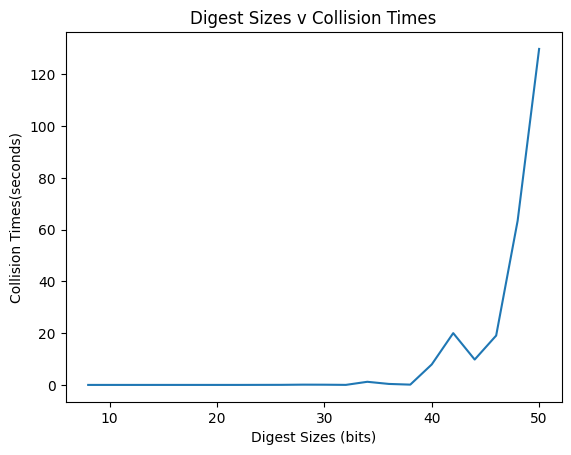
\includegraphics[width=0.5\textwidth]{./assets/digest_sizes_v_collision_times.png}
		\caption{Digest Size vs Time}
		\label{fig:collision_times}
	\end{subfigure}
	\begin{subfigure}{1.00\textwidth}
		\centering
		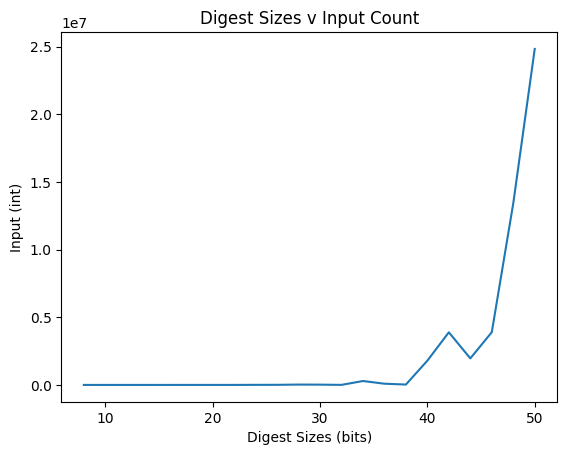
\includegraphics[width=0.5\textwidth]{./assets/digest_sizes_v_imput_count.png}
		\caption{Digest Size vs Input}
		\label{fig:collision_inputs}
	\end{subfigure}
	\caption{Collision Resistance}
	\label{fig:collision_performance}
\end{figure}

\subsubsection*{Code}
\begin{lstlisting}
# Truncates a digest to a particular
# to a particular domain (in bits)
def part_c(digest: bytes, trunc_len: int) -> bytes:
    # Bytes needed to remove from the digest 
    # working with bytearrays are easier
    truncate_bytes_count: int = trunc_len // 8
    # Remaining fine tuning bits to "remove"
    truncate_bits_count: int = trunc_len % 8

    # Take the first n bytes
    truncated_digest: bytearray = bytearray(digest[:truncate_bytes_count])

    # Bitshift the remaining bits from the digest and tack it on the end of the
    # truncated_digest
    if truncate_bits_count > 0:
        # Note that the remainder of the 'byte' is going to be just zeros
        mask: float = (0xFF << (8-truncate_bits_count)) & 0xFF
        last_byte: float = digest[truncate_bytes_count] & mask
        truncated_digest.append(last_byte)

    return bytes(truncated_digest)

# Takes advantage of the birthday problem 
def process_graphs(hash_obj: SHA256.SHA256Hash) -> None:
    asset_path: str = './assets' 
    dvc_path: str = os.path.join(asset_path, 'digest_sizes_v_collision_times.png')
    dvi_path: str = os.path.join(asset_path, 'digest_sizes_v_imput_count.png') 

    digest_sizes: list[int] = list(range(8, 51, 2))
    collision_times: list[float] = [] # in seconds
    input_count: list[int] = [] # in seconds

    # {truncated digest: message}
    seen: dict[bytes, bytes] = {}

    # =======================================================================

    for b in digest_sizes:
        start_time: float = time.perf_counter()
        j: int = 0

        while True:
            j += 1
           
            # changing the length of this inital input vector did not do that
            # much to help with the time
            m0_bytes: bytes = os.urandom(10)
            m0_digest: bytes = part_a(m0_bytes, hash_obj, False)
            m0_truncated_digest: bytes = part_c(m0_digest, b)
            
            if m0_truncated_digest in seen and m0_bytes != seen[m0_truncated_digest]:
                print(f'[{b}]Collision found at iteration {j} with digest: {m0_truncated_digest}')
                print(f'[{b}]message_0: {m0_bytes}')
                print(f'[{b}]message_1: {seen[m0_truncated_digest]}')
                print('-------------------------\n')

                elapsed_time: float = time.perf_counter() - start_time

                collision_times.append(elapsed_time)
                input_count.append(j)

                break # break the while loop
            else:
                # add it to the list of seen digests
                seen.update({m0_truncated_digest: m0_bytes})


    print(f'digest_sizes: {digest_sizes}')
    print(f'collision_times: {collision_times}')
    print(f'input_count: {input_count}')

    plt.plot(digest_sizes, collision_times)
    plt.xlabel('Digest Sizes (bits)')
    plt.ylabel('Collision Times(seconds)')
    plt.title('Digest Sizes v Collision Times')

    plt.savefig(dvc_path, bbox_inches='tight')
    # plt.show()

    plt.clf()

    plt.plot(digest_sizes, input_count)
    plt.xlabel('Digest Sizes (bits)')
    plt.ylabel('Input (int)')
    plt.title('Digest Sizes v Input Count')

    plt.savefig(dvi_path, bbox_inches='tight')
    # plt.show()

    plt.clf()
\end{lstlisting}

\subsection*{Main Code}
\begin{lstlisting}
if __name__ == '__main__':
    hash_obj: SHA256.SHA256Hash = SHA256.new()

    # Part A
    print('\n--- Task1 Part A ---\n')

    foo_a: bytes = 'Hello, World!'.encode('utf-8')
    part_a(foo_a, hash_obj)

    # Part B 
    print('\n--- Task1 Part B ---\n')

    str0: str = 'Hello'
    str1: str = 'beautiful'
    str2: str = 'world!'

    hashed_str0_original, hashed_str0_hammed = part_b(str0, hash_obj)
    print(f'Original Digest: {hashed_str0_original}')
    print(f'Hammed Digest:   {hashed_str0_hammed}\n')

    hashed_str1_original, hashed_str1_hammed = part_b(str1, hash_obj)
    print(f'Original Digest: {hashed_str1_original}')
    print(f'Hammed Digest:   {hashed_str1_hammed}\n')

    hashed_str2_original, hashed_str2_hammed = part_b(str2, hash_obj)
    print(f'Original Digest: {hashed_str2_original}')
    print(f'Hammed Digest:   {hashed_str2_hammed}\n')

    print('\n--- Task1 Part C ---\n')
    # Part C (option 1 because I am lazy...)
    process_graphs(hash_obj)
\end{lstlisting}

\section*{Environment}
If you want to run and test the code, a virtual environment should first be set up with the correct requirements. This ensures that there is consistency between all of the packages used within this project.

\begin{itemize}
	\item Make a virtual environment (venv) with Python.
		\verb|$ python3 -m venv .venv|
	\item Activate the venv.
		\verb|$ source .venv/bin/activate|
	\item Install the requirements using pip.
		\verb|$ pip install -r requirements.txt|
	\item Whenever you are done, you can deactivate the venv.
		\verb|$ deactivate|
\end{itemize}

\subsection*{Reproduction}
Running any of the code is as simple as activating the venv and then running the python script.

\verb|(.venv) python task3.py|

% ============================================================================
\section*{Task 2: Breaking Real Hashes}
\subsection*{Abstract}
This is what I did and how it works and blah blah blah

\subsection*{Code}

\begin{lstlisting}
printf("Hello, World!");
\end{lstlisting}

% ============================================================================

\section*{Questions}
\subsection*{Question 1}
Even though the original strings were offset by a difference of only one bit, it still drastically changed the digest. This is pretty reassuring; the output is not predictable, and it makes a very big difference.

\subsection*{Question 2}
For a hash with a fixed output size \verb|(n)|, by definition, the digest is 256 bits, where a bit can be either a 0 or a 1 (there are two options for every bit). This results in a maximum space of \verb|2\^n| different possibilities. Therefore, if you somehow managed to get \verb|2\^n| unique hashes, from \verb|2\^n| arbitrary inputs, then the next hash you take must map to a digest in the vector-space that has already been visited. So the maximum number of hashes needed to encounter a collision would have to be \verb|2\^n| (this is assuming you have hashed one fixed message, and try all other \verb|2\^n| combinations on a different input message). However, this is not what happens all of the time. The Birthday Paradox shows us that the expected number of files to guess in order to find a collision is \verb|2^(n/2)|.

Given the data that we collected (on Jude's laptop), the average time it took to process a single input was \verb|4.206261571130722e-06| seconds. If we stuck with the brute force method, we would calculate \verb|(2^256)*(4.206261571130722e-06)|, which comes out to \verb|4.889624740283841e+71| seconds, or \verb|1.5495 * 10^64| years. Even if we try to leverage the birthday problem, the average time would be \verb|(2^(256/2))*(4.206261571130722e-06)|, which comes out to \verb|1.4313166e+33| seconds, or \verb|4.5357 * 10^25| years. Both are insanely incomprehensible.

\subsection*{Question 3}
There are only \verb|2\^n|; if the digest size is 8 bits, then there are only 256 different possibilities to brute force through. Because of the birthday problem, the number of attempts to find a collision reduces down to \verb|2\^(8/2)|, which comes out to be 16 tries (significantly less). To be honest, both cases are relatively trivial to break.

The mapping from input to digest is one way, but inherritaly, there are going to be collisions because no hash is perfect. Because this is the case, there is a one to many relationship when trying to use a digest to get an input (or preimage). In this case, we are analyzing trying to find only the first preimage. 

\subsection*{Question 4}

\end{document}
